\documentclass[10pt,a4paper,conference]{IEEEtran}
\usepackage[utf8]{inputenc}
\usepackage[T1]{fontenc}
\usepackage[spanish,es-tabla]{babel}
\usepackage{newtxtext,newtxmath}
\usepackage{graphicx,booktabs,tabularx,array}
\usepackage{amsmath}
\usepackage[hidelinks]{hyperref}
\usepackage{xurl}
\usepackage{placeins,capt-of}
\renewcommand{\IEEEkeywordsname}{Palabras clave}
\urlstyle{same}
\setlength{\emergencystretch}{2em}
\newcolumntype{Y}{>{\raggedright\arraybackslash}X}
\title{Control de dos LED con Arduino UNO y un módulo HC-05 simulado}
\author{\IEEEauthorblockN{Leydi Adriana Martínez López, Christian David Lancheros Martínez,}
\IEEEauthorblockN{Verónica Mora Cerón, Juan Camilo Bellon y Danyela Vivian Munza Suárez}
\IEEEauthorblockA{Politécnico Grancolombiano\\Módulo Internet de las cosas\\
Docente Jesús Antonio Figueroa Guerrero\\
Entrega 2 --- Pruebas realizadas el 21 de noviembre de 2026}}
\begin{document}
\maketitle
\raggedbottom
\begin{abstract}
Se implementó y probó en Mokxi un circuito con Arduino UNO, un modelo del módulo HC-05 y dos LED con resistencias de 220 ohmios. Se adaptó el ejemplo Bluetooth lamp para controlar por separado las salidas verde y roja mediante comandos de texto. La comunicación con el módulo se configuró a 1200 baudios y el monitor serial de Arduino a 115200 baudios. Se documentaron el encendido y apagado individual, el apagado conjunto, la consulta del estado, el manejo de un comando inválido y la desconexión y recuperación del enlace simulado. Las capturas muestran respuestas coherentes con los estados observados de las salidas. El trabajo verifica la interfaz serial del modelo y el comportamiento del programa; no constituye una medición de la propagación, interferencia o seguridad de una conexión Bluetooth física.
\end{abstract}
\begin{IEEEkeywords}
Arduino UNO, HC-05, UART, comunicación serial, simulación, LED.
\end{IEEEkeywords}

\noindent\textbf{Abstract---}\textit{A circuit comprising an Arduino UNO, a simulated HC-05 module, and two LEDs with 220-ohm resistors was implemented and tested in Mokxi. The Bluetooth lamp example was adapted to control green and red outputs independently through text commands. The module interface operated at 1200 baud, while the Arduino serial monitor was initialized at 115200 baud. Tests covered individual switching, simultaneous shutdown, state reporting, invalid input, disconnection, and reconnection. Screenshots show replies consistent with the observed output states. The experiment validates the model's serial interface and program behavior, without measuring physical Bluetooth propagation, interference, or security.}

\noindent\textbf{Index Terms---}Arduino UNO, HC-05, UART, serial communication, simulation, LED.

\section{Introducción}
La segunda entrega de la guía Uso práctico de Arduino solicita implementar un montaje con recepción de señales por Bluetooth, configurar el enlace serial de la placa y documentar pruebas de conectividad en simulación. Su diagrama de referencia incluye Arduino, un módulo de comunicación y dos LED \cite{guia}. El objetivo de esta práctica fue reproducir esas funciones de control en un modelo ejecutable y registrar las respuestas de las salidas.

El trabajo inicial en Wokwi permitía controlar dos LED desde el monitor serial, pero su archivo de circuito no incluía el HC-05. Se conservó como antecedente de la lógica de comandos y se preparó un montaje final en Mokxi con el módulo explícito, dos salidas y un terminal que representa al dispositivo remoto. La evidencia de este artículo corresponde al montaje final; las capturas del ejemplo previo de una sola lámpara no se presentan como pruebas del circuito de dos LED.

\section{Fundamentos y revisión documental}
\subsection{Arduino y control de salidas}
Arduino UNO R3 utiliza el ATmega328P y dispone de entradas y salidas digitales programables \cite{uno}. En esta práctica, dos pines se configuran como salidas para representar estados binarios mediante LED. Una resistencia de 220~$\Omega$ se coloca en serie con cada LED. El programa mantiene variables separadas para las salidas verde y roja y modifica solo la salida solicitada, salvo el comando de apagado conjunto.

\subsection{Interfaz serial del HC-05}
El modelo HC-05 de Mokxi intercambia datos por los pines TXD y RXD y expone STATE para indicar la conexión lógica del terminal. La documentación describe tramas UART 8N1 y un panel Bluetooth que representa el extremo remoto. También delimita el modelo: no reproduce la propagación ni las interferencias de una radio física \cite{modelo}. Es necesario distinguir el emparejamiento mostrado por la interfaz del simulador de una asociación entre dispositivos físicos.

\subsection{Publicaciones científicas relacionadas}
Kondaveeti y colaboradores presentan una revisión sistemática de estudios sobre prototipado con Arduino, sus aplicaciones, ventajas, dificultades y limitaciones \cite{kondaveeti}. Ese trabajo permite situar el montaje en una actividad de prototipado y no únicamente en el uso de una herramienta de programación. Para esta práctica, la implicación metodológica es documentar qué se implementó, con qué configuración se evaluó y qué resultados respaldan las conclusiones. La referencia no demuestra por sí sola el funcionamiento del circuito del grupo; ese respaldo procede de las capturas y los archivos de esta entrega.

Sharkawy y colaboradores desarrollaron cinco aplicaciones de hogar inteligente con Arduino UNO R3, Android y un módulo HC-06. Su artículo describe los componentes, las conexiones, las interfaces de usuario y las pruebas de un montaje físico organizado sobre un panel; también ofrece material complementario \cite{sharkawy}. El caso resulta pertinente por el control de iluminación mediante un módulo serial Bluetooth. Sin embargo, utiliza HC-06 y hardware físico, mientras que esta entrega emplea un modelo HC-05 y LED virtuales. Por ello, sus resultados no se transfieren como mediciones del presente trabajo.

Ambas publicaciones aportan una base investigativa que complementa las fichas del fabricante y la documentación del simulador. La revisión se concentra en el prototipado y el control local: no pretende demostrar una conexión a Internet, una revisión exhaustiva de la literatura ni el desempeño de una radio real.

\subsection{Ejemplo de partida y adaptación}
El circuito y las rutinas de transmisión y recepción por software se tomaron del ejemplo Bluetooth lamp de Mokxi \cite{ejemplo}. Se reconoce esa procedencia: no se atribuye al grupo la creación del simulador ni la autoría original de las rutinas UART. La adaptación añadió la rama del LED rojo, cambió la lámpara original por un LED verde y sustituyó los comandos del ejemplo por los del control de dos salidas. Se añadieron la consulta de ambos estados y el rechazo de líneas demasiado largas.

\section{Implementación y configuración}
\subsection{Componentes y conexiones}
Se emplearon una placa UNO, una protoboard, un HC-05, dos LED y dos resistencias. La Tabla~\ref{tab:pines} resume las conexiones funcionales. Los negativos de las ramas y del módulo comparten tierra. En la protoboard, las uniones internas completan cada rama entre la resistencia, el ánodo y el cátodo del LED.

\begin{table}[htbp]
\caption{Conexiones funcionales del montaje final}
\label{tab:pines}
\centering\footnotesize
\begin{tabularx}{\columnwidth}{@{}lY@{}}
\toprule
Elemento & Conexión en Arduino UNO \\
\midrule
HC-05 VCC y GND & 5V y GND, mediante los rieles de alimentación \\
HC-05 TXD & D2, recepción UART por software \\
HC-05 RXD & D3, transmisión UART por software \\
HC-05 STATE & D4, entrada de estado del enlace \\
LED verde & D9, resistencia de 220~$\Omega$, ánodo y cátodo a GND \\
LED rojo & D10, resistencia de 220~$\Omega$, ánodo y cátodo a GND \\
\bottomrule
\end{tabularx}
\end{table}

La conexión directa de D3 al RXD corresponde al ejemplo simulado. Para trasladar el montaje a hardware debe verificarse la hoja de datos de la placa HC-05 utilizada y la adaptación de niveles de esa entrada; el simulador no valida daño eléctrico \cite{modelo}. No se construyó ni ensayó un montaje físico.

\subsection{Dos enlaces seriales diferentes}
El HC-05 se configuró con la propiedad \texttt{baud=1200}. El código utiliza \texttt{BIT\_US=833}, aproximación del período de bit:
\begin{equation}
T_{bit}=\frac{1}{1200}\ \mathrm{s}\approx833{,}3\ \mu\mathrm{s}.
\end{equation}
Las funciones \texttt{readByte()} y \texttt{writeByte()} realizan el muestreo y la transmisión mediante operaciones digitales y esperas en microsegundos. El receptor comprueba que el bit de parada sea alto. Estas rutinas se conservaron del ejemplo que se probó inicialmente.

Por separado, \texttt{Serial.begin(115200)} inicializa el puerto de diagnóstico de Arduino. Esa llamada no configura la UART implementada en D2 y D3. Por ello, los 115200 baudios del monitor y los 1200 baudios del módulo no son una contradicción: pertenecen a canales diferentes. Los mensajes enviados por el terminal HC-05 se finalizan con CR+LF.

\subsection{Procesamiento de comandos}
El programa acumula texto hasta recibir un retorno de carro o salto de línea. Después compara la línea completa con los comandos de la Tabla~\ref{tab:comandos}. Las mayúsculas y minúsculas tienen significado distinto. El retorno adicional de CR+LF no ejecuta otro comando, porque una línea vacía se ignora. El arreglo de entrada tiene 24 posiciones: admite hasta 23 caracteres y un terminador. Si se supera ese límite se devuelve un aviso; esa condición no se incluyó en las pruebas capturadas.

\begin{table}[htbp]
\caption{Protocolo de comandos del circuito final}
\label{tab:comandos}
\centering\footnotesize
\begin{tabularx}{\columnwidth}{@{}lYY@{}}
\toprule
Comando & Acción & Respuesta \\
\midrule
\texttt{V} & Encender verde & \texttt{Verde ON} \\
\texttt{v} & Apagar verde & \texttt{Verde OFF} \\
\texttt{R} & Encender rojo & \texttt{Rojo ON} \\
\texttt{r} & Apagar rojo & \texttt{Rojo OFF} \\
\texttt{A} & Apagar ambos & \texttt{Ambos OFF} \\
\texttt{status} & Consultar ambos estados & Estado de verde y rojo \\
Otro texto & Mantener las salidas & \texttt{Comando invalido} \\
\bottomrule
\end{tabularx}
\end{table}

Cada respuesta se envía al módulo únicamente si STATE indica conexión. La rutina de diagnóstico escribe también el comando recibido por el puerto serial de Arduino. El uso de esperas para cada bit significa que este firmware no es totalmente no bloqueante. No se realizaron pruebas de tráfico concurrente ni de saturación.

\subsection{Procedimiento de simulación}
Se importó el archivo nativo \path{Entrega2_HC05_dos_LED.mokxi.json} mediante \textit{Open JSON or SPICE}. Este archivo conserva el módulo, las conexiones y el programa. Se inició \textit{Run}, se abrió el panel Bluetooth y se conectó el terminal al HC-05. La interfaz confirmó 1200 baudios. Los comandos se enviaron de forma manual, uno por vez, conservando CR+LF.

Se verificaron las respuestas de texto y el brillo de los LED. Se capturaron encendido verde, encendido rojo con el verde aún activo, apagados individuales y apagado conjunto. A continuación se consultó el estado, se envió un texto inválido y se ejecutaron desconexión y reconexión desde la interfaz.

\section{Resultados y análisis}
La Tabla~\ref{tab:resultados} reúne las observaciones del circuito de dos LED. Las Figuras~\ref{fig:verde} a~\ref{fig:recuperacion} presentan recortes de las capturas aportadas durante las pruebas. Los recortes reúnen el circuito y el terminal de una misma captura, omitiendo paneles vacíos; no se modificaron los mensajes ni los estados visibles. Los originales se conservan en los archivos de evidencia.

\begin{table}[htbp]
\caption{Resultados observados en la secuencia de pruebas}
\label{tab:resultados}
\centering\footnotesize
\begin{tabularx}{\columnwidth}{@{}lYY@{}}
\toprule
Prueba & Respuesta visible & Estado observado \\
\midrule
\texttt{V} & Verde ON & Solo verde encendido \\
\texttt{R} & Rojo ON & Ambos encendidos \\
\texttt{v} & Verde OFF & Solo rojo encendido \\
\texttt{r} & Rojo OFF & Ambos apagados \\
\texttt{A}, tras V y R & Ambos OFF & Ambos apagados \\
\texttt{status} & Verde OFF Rojo OFF & Coincide con las salidas \\
\texttt{hola} & Comando invalido & Ambos siguen apagados \\
Desconexión & the phone disconnected & Entrada: Connect first \\
Reconexión y V & connected; Verde ON & Verde vuelve a encender \\
\bottomrule
\end{tabularx}
\end{table}

Los comandos individuales permitieron modificar una salida conservando la otra. Al enviar \texttt{R} después de \texttt{V}, ambas permanecieron encendidas. Al enviar \texttt{v}, el rojo permaneció activo. La consulta \texttt{status}, realizada después de \texttt{A}, devolvió ambos estados apagados. La entrada \texttt{hola} fue rechazada y no modificó las salidas.

La desconexión dejó el dispositivo emparejado en la interfaz, pero sin un enlace activo: se mostró \textit{Connect first} en el campo de envío. Al pulsar \textit{Connect} y transmitir \texttt{V}, se recibió nuevamente \texttt{Verde ON}. Esto acredita recuperación funcional del enlace lógico dentro del simulador.

No se midieron retardos entre el envío y la respuesta, pérdida de paquetes ni tasa máxima de comandos. Las capturas son observaciones funcionales y no una prueba estadística de confiabilidad. El montaje anterior de Wokwi registraba intervalos entre comandos mediante \texttt{millis()}; esos intervalos no equivalen a latencia Bluetooth y no se reutilizan como mediciones del circuito final.

\subsection{Repetición y control experimental}
Las nueve evidencias corresponden a una secuencia manual de verificación funcional. No son nueve corridas independientes ni un muestreo periódico. No se registraron intervalos uniformes, una distribución de latencias o indicadores del proceso del simulador; por tanto, no se calculan medias, desviaciones ni porcentajes de confiabilidad a partir de esas capturas.

Para ampliar el experimento se propone realizar tres corridas desde un reinicio, con el mismo equipo, navegador y archivo nativo. En cada corrida se enviaría cinco veces la secuencia V, R, v, r, V, R, A, status y hola, con una cadencia fijada previamente de cinco segundos entre envíos y espera de la respuesta antes del siguiente. Esto produciría 45 envíos por corrida y 135 en total. Debe anotarse el intervalo real observado, cualquier desviación de la cadencia y los casos sin respuesta; el número de envíos propuesto no representa datos ya obtenidos.

El registro debe conservar corrida, secuencia, comando, marca temporal de envío, marca de respuesta, estado esperado, estado observado e incidencias. Si se monitorea el computador, se debe identificar el proceso de la pestaña del simulador, registrar su identificador y muestrear CPU y memoria a intervalos constantes. Los totales de Windows no aíslan el consumo del simulador. Este seguimiento sería un experimento adicional: no se incorporan resultados de CPU o RAM sin mediciones originales.

\section{Alcance y limitaciones}
La evidencia demuestra el control de dos salidas, el intercambio de comandos y respuestas por el HC-05 modelado y el manejo de una desconexión desde la interfaz. El diálogo de PIN y las indicaciones \textit{Paired} y \textit{Connected} corresponden a estados de la aplicación. No se conectó un teléfono físico ni se verificó una pila de radio real.

La diferencia con el diagrama de referencia se documenta mediante la asignación de pines, las dos velocidades y el protocolo utilizado. El trabajo aporta una representación funcional del módulo y de la interfaz serial, sin afirmar equivalencia con una validación física completa. La evaluación de esa representación frente al requisito Bluetooth de la guía corresponde al alcance establecido por el docente.

\section{Conclusiones}
El montaje simulado permitió controlar de forma independiente dos LED y apagarlos conjuntamente. Las respuestas de los comandos probados coincidieron con los estados visibles de las salidas. La consulta del estado y el rechazo del texto inválido hicieron explícita la interacción entre el terminal y el programa.

La separación entre la UART del módulo a 1200 baudios y el puerto de diagnóstico a 115200 baudios evita confundir configuraciones de canales distintos. La desconexión y posterior respuesta al comando de encendido mostraron recuperación del enlace lógico simulado.

El archivo nativo conserva el circuito completo y el programa adaptado. La exportación para Wokwi excluye el HC-05, según el README de esa exportación, por lo que no se utiliza como archivo reproducible principal. El ejemplo de Mokxi se reconoce como fuente del montaje de partida y de las rutinas UART. Como trabajo posterior queda contrastar el comportamiento con hardware y medir desempeño bajo un protocolo experimental específico.

\section*{Disponibilidad de archivos}
El material complementario reúne el proyecto nativo \texttt{.mokxi.json}, el código \texttt{.ino}, las capturas originales y este artículo con sus fuentes LaTeX. Para reproducir el circuito se debe abrir el JSON nativo en Mokxi. El repositorio público y el circuito guardado se identifican mediante los siguientes enlaces. El archivo nativo se conserva para reproducir el montaje desde la configuración.

\noindent\textit{Repositorio público:} \url{https://github.com/martinezlopezleydi29-png/entrega2-iot-arduino-bluetooth}.

\noindent\textit{Circuito de dos LED:} \url{https://app.mokxi.com/p/WYKZzVkyr_cD1bT1}.



\FloatBarrier
\section*{Evidencias del circuito final}
\noindent Las siguientes figuras documentan las pruebas manuales del 21 de noviembre de 2026. Se conservan las capturas completas en la carpeta de evidencias. La presentación del artículo usa la clase IEEEtran para conferencias, disponible entre las herramientas de formato IEEE \cite{ieee}.
\par\medskip\noindent\begin{minipage}{\columnwidth}
\centering
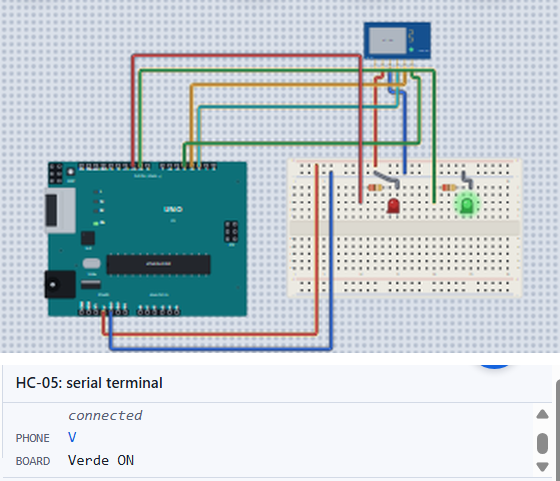
\includegraphics[width=\columnwidth]{imagenes/verde.png}
\captionof{figure}{Encendido del LED verde tras enviar V. El LED rojo permanece apagado.}
\label{fig:verde}
\end{minipage}\par\medskip

\par\medskip\noindent\begin{minipage}{\columnwidth}
\centering
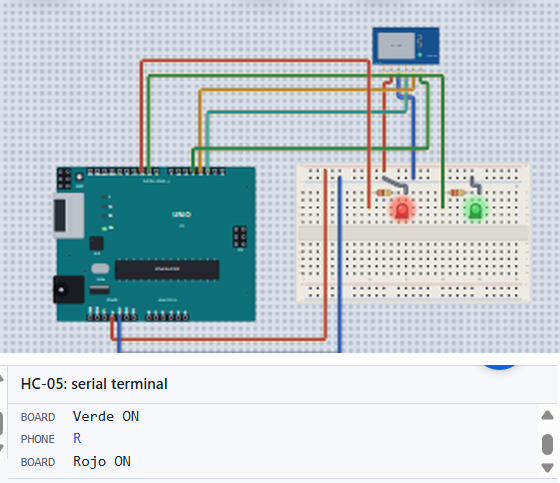
\includegraphics[width=\columnwidth]{imagenes/ambos.png}
\captionof{figure}{Encendido del LED rojo tras enviar R, conservando el verde encendido.}
\label{fig:ambos}
\end{minipage}\par\medskip

\par\medskip\noindent\begin{minipage}{\columnwidth}
\centering
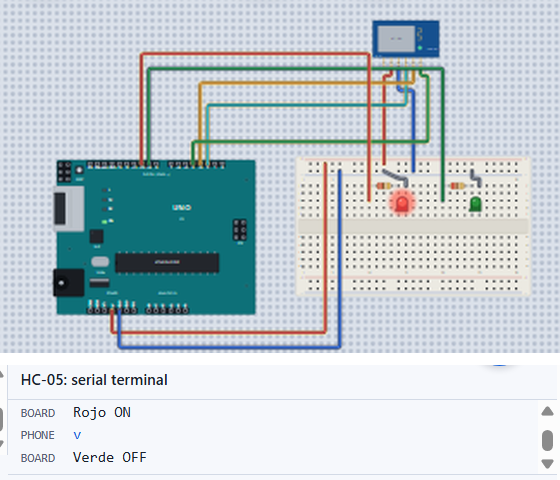
\includegraphics[width=\columnwidth]{imagenes/solo_rojo.png}
\captionof{figure}{Apagado del verde mediante v. El rojo permanece encendido.}
\label{fig:solo_rojo}
\end{minipage}\par\medskip

\par\medskip\noindent\begin{minipage}{\columnwidth}
\centering
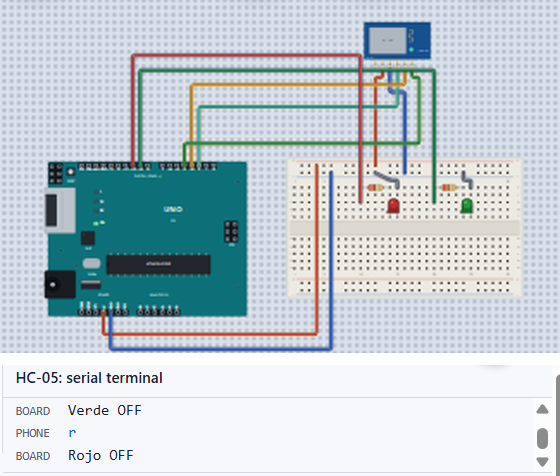
\includegraphics[width=\columnwidth]{imagenes/apagados.png}
\captionof{figure}{Apagado del rojo mediante r. Ambas salidas quedan apagadas.}
\label{fig:apagados}
\end{minipage}\par\medskip

\par\medskip\noindent\begin{minipage}{\columnwidth}
\centering
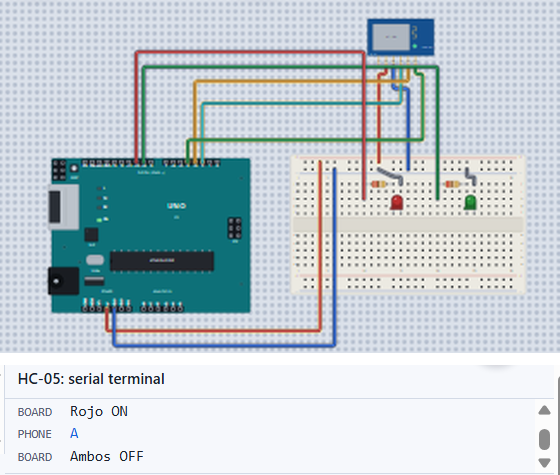
\includegraphics[width=\columnwidth]{imagenes/apagar_todo.png}
\captionof{figure}{Apagado conjunto mediante A. El registro anterior muestra Rojo ON.}
\label{fig:apagar_todo}
\end{minipage}\par\medskip

\par\medskip\noindent\begin{minipage}{\columnwidth}
\centering
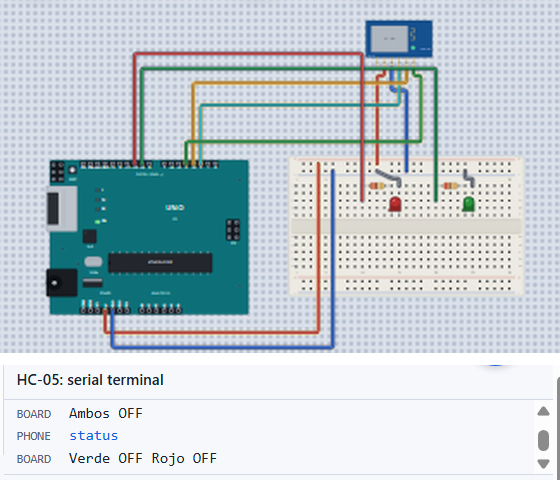
\includegraphics[width=\columnwidth]{imagenes/estado.png}
\captionof{figure}{Consulta status después del apagado conjunto. La respuesta indica ambos LED apagados.}
\label{fig:estado}
\end{minipage}\par\medskip

\par\medskip\noindent\begin{minipage}{\columnwidth}
\centering
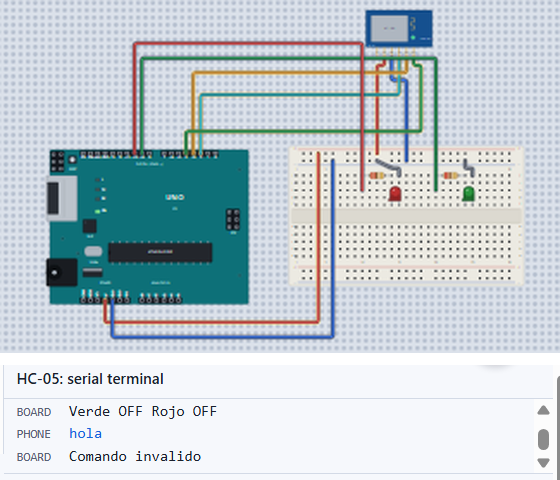
\includegraphics[width=\columnwidth]{imagenes/invalido.png}
\captionof{figure}{Rechazo de hola con la respuesta Comando invalido y sin encender las salidas.}
\label{fig:invalido}
\end{minipage}\par\medskip

\par\medskip\noindent\begin{minipage}{\columnwidth}
\centering
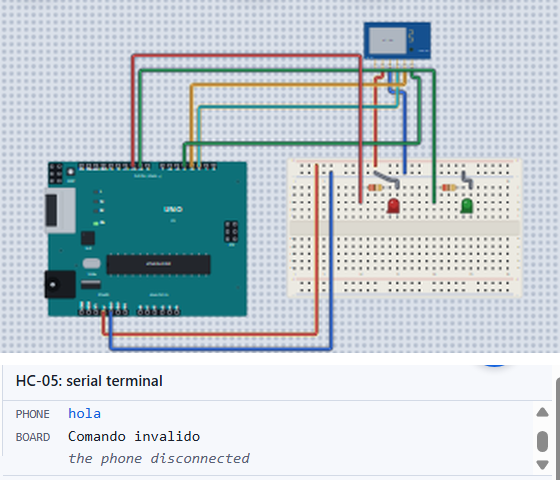
\includegraphics[width=\columnwidth]{imagenes/desconexion.png}
\captionof{figure}{La terminal registra the phone disconnected tras la desconexión del enlace simulado.}
\label{fig:desconexion}
\end{minipage}\par\medskip

\par\medskip\noindent\begin{minipage}{\columnwidth}
\centering
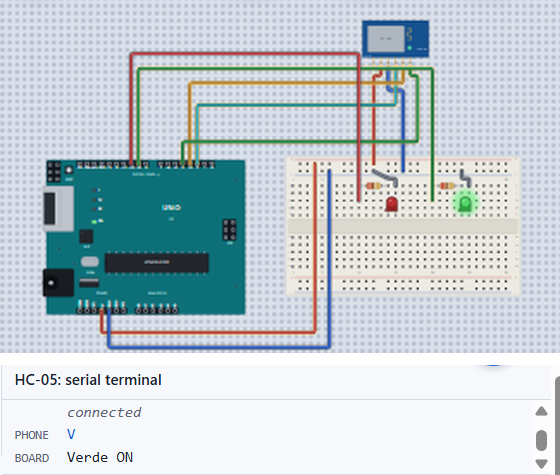
\includegraphics[width=\columnwidth]{imagenes/recuperacion.png}
\captionof{figure}{Tras conectar de nuevo, el comando V recibe Verde ON y el LED verde se enciende.}
\label{fig:recuperacion}
\end{minipage}\par\medskip

\begin{thebibliography}{7}
\bibitem{guia} Politécnico Grancolombiano, \textit{Uso práctico de Arduino}, guía del módulo Internet de las cosas, entrega 2, p.~5, s.~f.
\bibitem{uno} Arduino, ``UNO R3,'' documentación de hardware. [En línea]. Disponible en: \url{https://docs.arduino.cc/hardware/uno-rev3/}. Consulta: 21 nov. 2026.
\bibitem{modelo} Mokxi, ``The HC-05 and HC-06, honestly,'' documentación del modelo. [En línea]. Disponible en: \url{https://mokxi.com/docs/parts/wireless-serial}. Consulta: 21 nov. 2026.
\bibitem{kondaveeti} H. K. Kondaveeti, N. K. Kumaravelu, S. D. Vanambathina, S. E. Mathe y S. Vappangi, ``A systematic literature review on prototyping with Arduino: Applications, challenges, advantages, and limitations,'' \textit{Computer Science Review}, vol. 40, art. 100364, 2021, doi: \href{https://doi.org/10.1016/j.cosrev.2021.100364}{10.1016/j.cosrev.2021.100364}.
\bibitem{sharkawy} A.-N. Sharkawy, M. Hasanin, M. Sharf, M. Mohamed y A. Elsheikh, ``Development of Smart Home Applications Based on Arduino and Android Platforms: An Experimental Work,'' \textit{Automation}, vol. 3, no. 4, pp. 579--595, 2022, doi: \href{https://doi.org/10.3390/automation3040029}{10.3390/automation3040029}.
\bibitem{ejemplo} Mokxi, ``Bluetooth lamp on an Arduino Uno: code and parts,'' ejemplo de partida. [En línea]. Disponible en: \url{https://mokxi.com/projects/bluetooth-lamp}. Consulta: 21 nov. 2026.
\bibitem{ieee} IEEE, ``Authoring Tools and Templates,'' IEEE Author Center Conferences. [En línea]. Disponible en: \url{https://conferences.ieeeauthorcenter.ieee.org/write-your-paper/authoring-tools-and-templates/}. Consulta: 21 nov. 2026.
\end{thebibliography}
\end{document}
